\documentclass[border=10pt]{standalone}
\usepackage[svgnames]{xcolor}
\usepackage{amsmath}
\usepackage{pgfplots}
\pgfplotsset{compat=newest}
\usepackage[sfdefault]{FiraSans}
\usepackage{FiraMono}
\renewcommand*\familydefault{\sfdefault}
\begin{document}
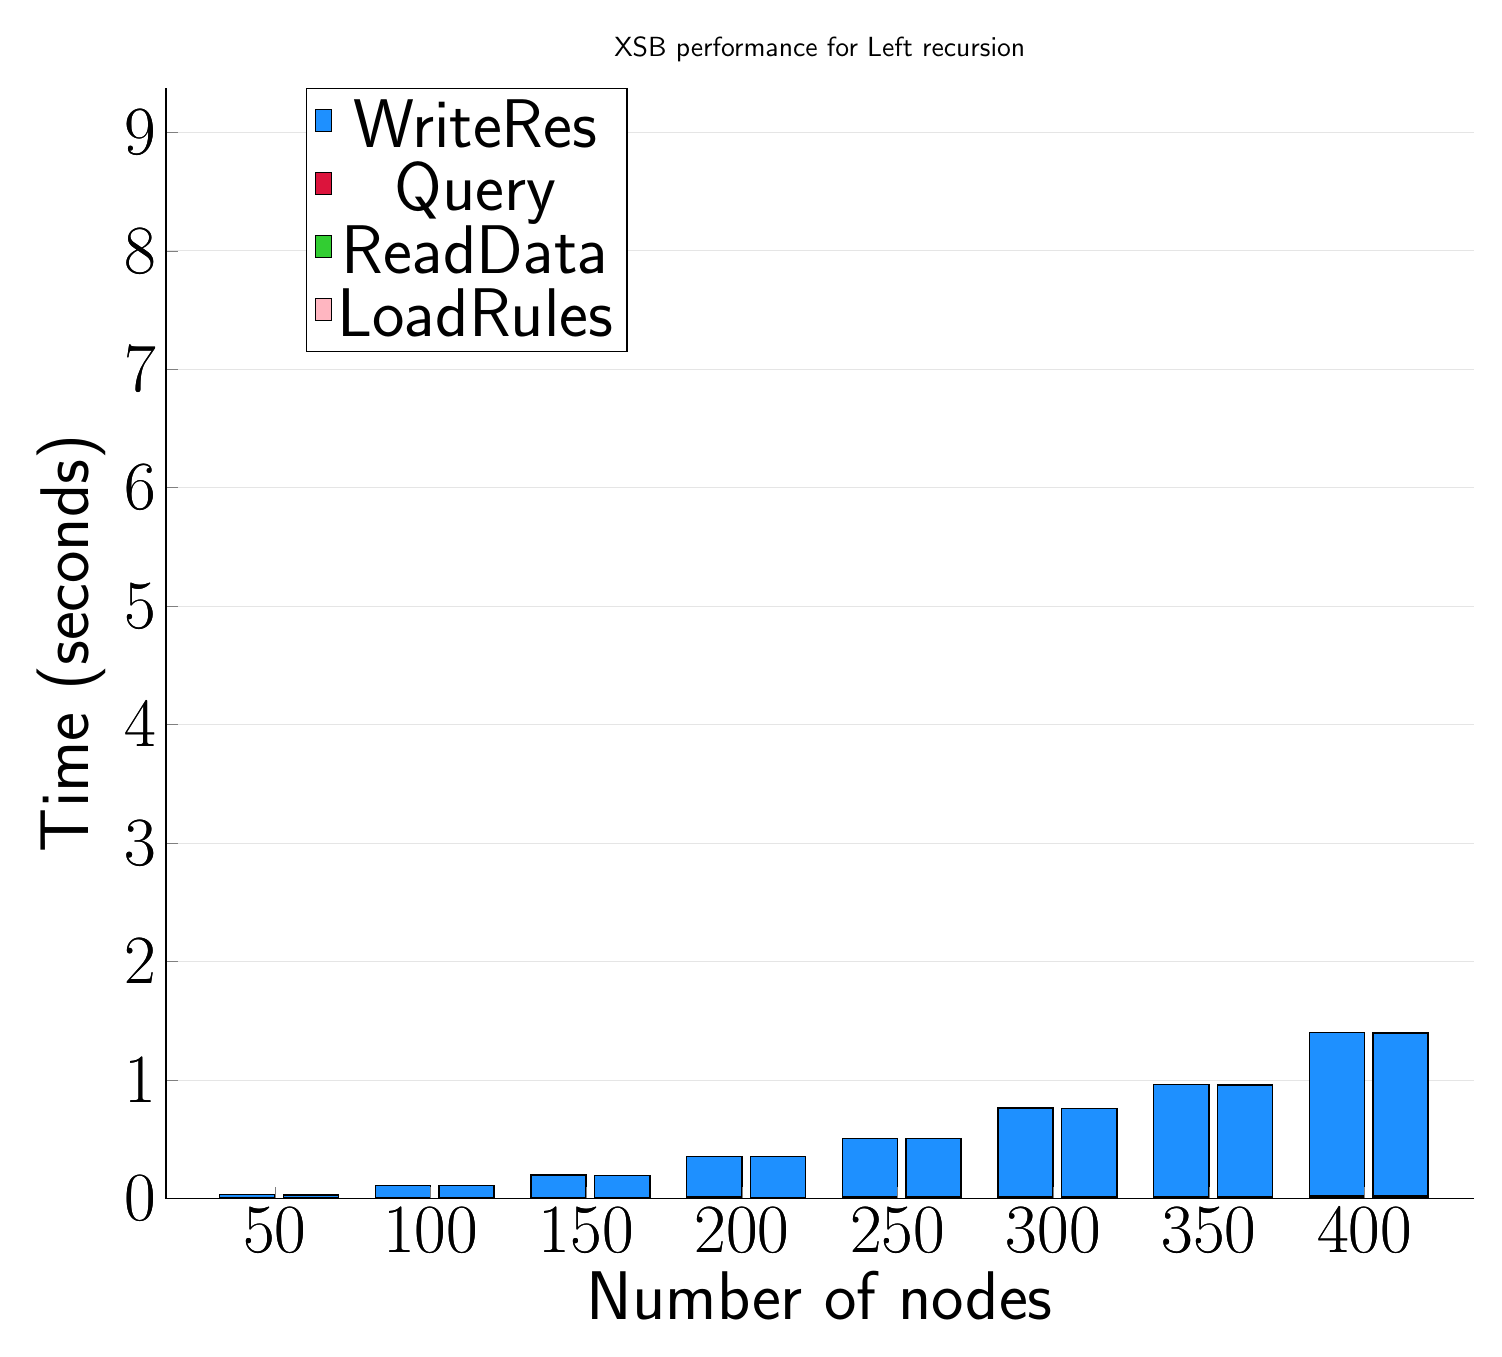
\begin{tikzpicture}
\begin{axis}[
   ybar stacked,
   title={XSB performance for Left recursion},
   bar shift=-10pt,
   width=1.5\textwidth,
   bar width=0.7cm,
   ymajorgrids, tick align=inside,
   major grid style={draw=gray!20},
   xtick=data,
   ymin=0, ymax=9.375487327575684,
   axis x line*=bottom,
   axis y line*=left,
   enlarge x limits=0.1,
   legend style={
       at={(0.23, 1)},
       anchor=north,
       legend columns=1,
       font=\Huge,
   },
   ylabel={Time (seconds)},
   xlabel={Number of nodes},
   label style={font=\Huge},
   tick label style={font=\Huge},
]
\addlegendimage{fill=DodgerBlue, draw=black, line width=0.2pt}
\addlegendentry{WriteRes}
\addlegendimage{fill=Crimson, draw=black, line width=0.2pt}
\addlegendentry{Query}
\addlegendimage{fill=LimeGreen, draw=black, line width=0.2pt}
\addlegendentry{ReadData}
\addlegendimage{fill=LightPink, draw=black, line width=0.2pt}
\addlegendentry{LoadRules}
\addplot +[fill=LightPink, draw=black, line width=0.5pt] coordinates {
    (50, 0.004170735677083333)
    (100, 0.0036199092864990234)
    (150, 0.00342273712158203)
    (200, 0.0035090446472167934)
    (250, 0.0035449663798014334)
    (300, 0.0035249392191569035)
    (350, 0.0036323865254720036)
    (400, 0.0034443537394205736)
};
\addplot +[fill=LimeGreen, draw=black, line width=0.5pt] coordinates {
    (50, 0.004726648330688493)
    (100, 0.0044496059417724635)
    (150, 0.0039122104644775365)
    (200, 0.005004008611043297)
    (250, 0.005707661310831703)
    (300, 0.0067267417907714835)
    (350, 0.0075010458628336565)
    (400, 0.009148995081583657)
};
\addplot +[fill=Crimson, draw=black, line width=0.5pt] coordinates {
    (50, 0.00023770332336425768)
    (100, 0.0008583863576253252)
    (150, 0.0017393430074056002)
    (200, 0.0031950473785400404)
    (250, 0.00439929962158203)
    (300, 0.006384372711181641)
    (350, 0.008551597595214842)
    (400, 0.013502995173136365)
};
\addplot +[fill=DodgerBlue, draw=black, line width=0.5pt] coordinates {
    (50, 0.027660687764485676)
    (100, 0.10230755805969244)
    (150, 0.19138129552205407)
    (200, 0.34395869572957327)
    (250, 0.4957465330759683)
    (300, 0.7484783331553144)
    (350, 0.9427817662556964)
    (400, 1.3754873275756836)
};
\end{axis}
\begin{axis}[
   ybar stacked,
   bar shift=13pt,
   width=1.5\textwidth,
   bar width=0.7cm,
   ymajorgrids, tick align=inside,
   major grid style={draw=none},
   xtick=data,
   ymin=0, ymax=9.375487327575684,
   axis x line*=none,
   axis y line*=none,
   enlarge x limits=0.1,
   label style={font=\Huge},
   tick label style={font=\Huge},
]
\addplot +[fill=LightPink, draw=black, line width=0.5pt] coordinates {
    (50, 0.0032606666666666665)
    (100, 0.0032133333333333337)
    (150, 0.002800333333333333)
    (200, 0.002263)
    (250, 0.002668666666666667)
    (300, 0.002526333333333333)
    (350, 0.0035923333333333332)
    (400, 0.0034436666666666665)
};
\addplot +[fill=LimeGreen, draw=black, line width=0.5pt] coordinates {
    (50, 0.0012826666666666663)
    (100, 0.0026130000000000003)
    (150, 0.0032823333333333333)
    (200, 0.004690333333333334)
    (250, 0.005468666666666666)
    (300, 0.005395333333333333)
    (350, 0.0073149999999999995)
    (400, 0.00901066666666666)
};
\addplot +[fill=Crimson, draw=black, line width=0.5pt] coordinates {
    (50, 0.00015066666666666465)
    (100, 0.000766333333333334)
    (150, 0.0015393333333333333)
    (200, 0.003161666666666667)
    (250, 0.004079333333333337)
    (300, 0.006049333333333334)
    (350, 0.008550666666666666)
    (400, 0.013493333333333335)
};
\addplot +[fill=DodgerBlue, draw=black, line width=0.5pt] coordinates {
    (50, 0.02644366666666667)
    (100, 0.102393)
    (150, 0.18811666666666663)
    (200, 0.3426403333333334)
    (250, 0.4947473333333334)
    (300, 0.7448043333333333)
    (350, 0.94062)
    (400, 1.3726166666666666)
};
\end{axis}
\end{tikzpicture}

\end{document}
